\section{Decentralized Supply Chain Management System} \label{usecase} 
The main contribution of this thesis is a decentralized Supply Chain Management and Shipment Tracker System. This system is proof of concept implementation to explore applications of blockchain for decentralized Supply Chain Management. As discussed in chapter \ref{TS} the backbone of our system is an Ethereum based Smart Contract. This contract allows invaluable and real time insight into the state of goods at every step of the delivery process. The logistical data is gathered using IoT based smart packages and communicated directly to the smart contract. The requirements for our system are derived from the use case presented in section \ref{ST-Dapp-UC}, so as to define realistic goals which could be realized in the given timeframe.

\vspace{0.5cm}
\subsection{Use Case Description} \label{ST-Dapp-UC} 
We take the example of an organization that has several suppliers around the world. It uses these suppliers to deliver different components and packages to its factory floor. These packages must be delivered on time and have to be stored, handled and transported under specific environmental or physical constraints. The organization and suppliers set up a business contract detailing delivery conditions. The business contract stipulates guarantees about delivery time and the conditions according to which the package needs to be handled, for example: At no point should the package be exposed to temperatures above a certain threshold.  This business use case is modeled in figure \ref{fig:UseCase}. The handling constraints are instantiated as requirements in the Smart Contract. Once requirements are set the Smart Contract behaves independently from the perspective of the shippers. This is shown in the figure \ref{fig:UseCase} by modeling the two instantiations as independent contracts i.e. Smart Contract A.1 and Smart Contract A.2. We will refer to them as SC-A.1 and SC-A from here on. Smart Contracts insure trust less compliance of the agreed upon terms and conditions. Payment channels are established between the organization and its suppliers to insure friction less payments and remunerations. In this case two payment channels exist, Payment Channel A between organization and Supplier A and Payment Channel B between organization and Supplier B as shown in figure \ref{fig:UseCase}. These will be referred to as PC-A and PC-B from here on. The system can further be extended to have payment channels between suppliers and shippers as shown in the use case diagram. These are modeled as Payment Channels C and D. These will be referred to as PC-C and PC-D. The organization is responsible for compensating every actor in the Supply Chain Life Cycle. In order to do so it can either use Ethereal or issue its own ERC20 tokens which can be exchanged for Eth. The main advantage of issuing your own ERC20 token is that you can fix the exchange rate so it’s always tied to a fixed Fiat value. This will protect against price fluctuations in Cryptocurrency value. All payment channels for a particular supply chain cycle use the same token. The suppliers and shippers get payed in ERC20 tokens.
%UseCase
\begin{figure}[h]
	\centering
    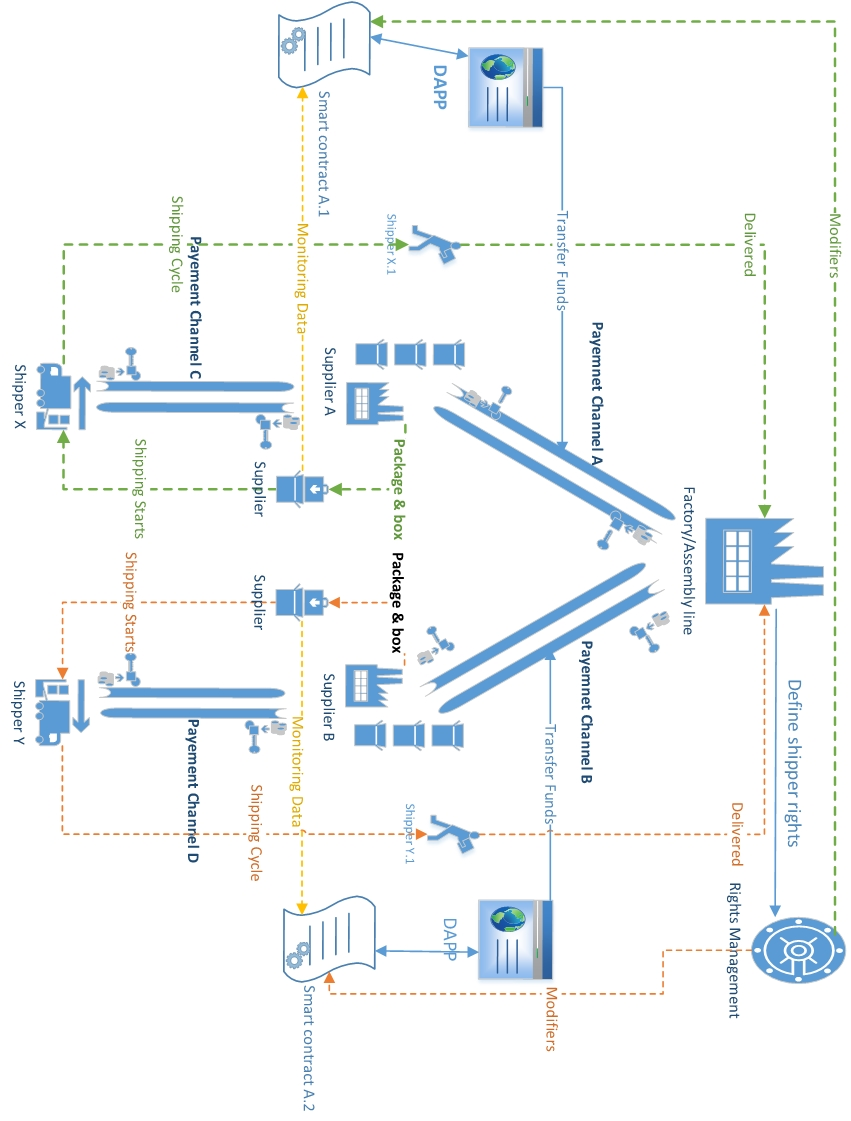
\includegraphics[width=180mm,scale=1]{figs/AbstractUC-flip}
	\caption{Shipment Tracker - Use case diagram}
	\label{fig:UseCase}
\end{figure}

\clearpage

%%%%%%Reminder: paper written use case docs is better then formal use case document I sent to the professor : rewrite and improve formal document using your paper notes

%\subsection{system Model \ requirements and assumptions} 
\subsubsection{Supply Chain LifeCycle}
To better explain the supply chain life cycle of our use case we use the simplified version of the system presented in figure \ref{fig:monitoring_subdiag}. This simplified version consists of only one supplier and shipper. The company places a new order for components with its supplier and stipulates shipping and handling constraints in the smart contract. 

\begin{figure}[h]
	\centering
    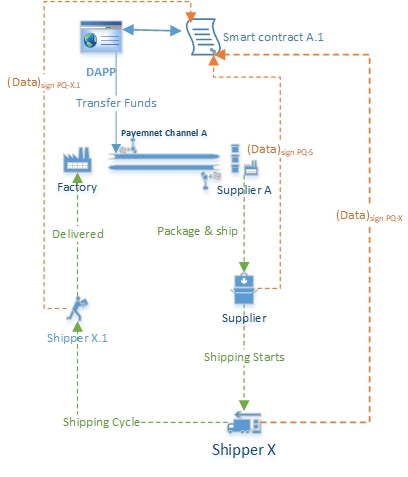
\includegraphics[width=140mm,scale=1]{figs/monitoring_subdiag}
	\caption{Supply Chain Life Cycle}
	\label{fig:monitoring_subdiag} 
\end{figure}
%\clearpage

Once the order has been placed it funds the payment channel associated with its supplier. Supplier packages the components along with a tamper proof smart device, which will communicate shipping data with the Smart Contract. The smart device is a Raspberry PI running a custom program developed as part of this thesis to monitor package conditions and to send signed data to the Smart Contract. 

The data can be signed with the help of a lattice based Post Quantum secure algorithm developed at TU Darmstadt. This algorithm protects integrity of data in the presence of post quantum adversaries. The hardware and software that collectively define a smart package will hence forth be referred to as the IoT Node. This node can be configured to send data continuously or when special events are triggered i.e. some shipping violation has occurred. We need internet connectivity throughout the shipping life cycle in order to insure monitoring data is continuously communicated with the Smart Contract and IPFS. The IoT Node signs the data with the Post Quantum key of the current shipper/ handler.  Monitoring starts as soon as the components are packaged in the supplier warehouse. At this time the data sent to the SC-A.1 is signed with key of the supplier. When the Shipper X takes possession of the package from the supplier they scan the package. This scanning event represents changing of ownership of responsibility in the Supply Chain Cycle, which means from this point on all data sent to the Smart Contract will be signed with the key of the Shipper X. If there is more than one shipper as show in figure \ref{fig:UseCase}, each one scans the package to take over shipping responsibilities. In our system Smart Contracts and Dapps are responsible for catching violations and taking appropriate actions to penalize violators and compensate aggrieved parties. This brings full transparency for all stake holders involved in the Supply Chain Cycle and resolves disputes in an efficient and trust less manner.

\vspace{0.5cm}
\subsection{System Architecture}
The proposed system for the use case described in \ref{ST-Dapp-UC} has four main components:
\begin{enumerate}
  \item Ethereum Smart Contract
  \item Raiden Payment Channels
  \item Decentralized Application or Master Nodes
  \item Smart packages or IoT Nodes
\end{enumerate} 

The abstract system and processes are modeled in figure \ref{fig:Abstractdesign}. Supplier and company agree on shipment conditions in the form of a business contract. These conditions are configured at the start of each shipment cycle. They are instantiated as requirements in a Smart Contract on the Ethereum blockchain. They cannot be altered after being set in the Smart Contract. The terms of the contract can include any type of handling constraints like exposure to high temperature, pressure, air etc. IoT enabled packages monitor (see \ref{IoT-Nodes}) the package contents with the help of embedded sensors. They communicate shipping and logistics data with the Smart Contract. The high level functions of IoT Node or Smart Package are modeled in the abstract design diagram shown in figure \ref{fig:Abstractdesign}.
\clearpage
The Smart Contract can detect any breaches of the agreed upon terms. If any breaches are detected the system can be used to take appropriate actions to compensate or penalize the parties involved. Payment Channels are established between the organization and its suppliers to handle payments efficiently. The payment channels are deployed using Raiden. A company and its suppliers agree upon a set of conditions either implicitly or explicitly at the start of each shipping cycle. The terms of conditions are instantiated in the contract with the help of contract number or tracking number of the package. The supplier initializes the IoT module inside smart package with the tracking number. Once initialized this module contacts the Smart Contract to receive set of conditions associated with the tracking number. The IoT Node starts the monitoring procedure as shown in figure \ref{fig:Abstractdesign}. To reduce operational costs only violations are stored in the blockchain. Full tracking logs containing sensor data like temperature, location, humidity etc. are stored using IPFS. The log address or Hash is stored in the blockchain. This enables our Dapp to always have access to complete logs.
%Once the package is delivered the organization can check the Dapp interface to see if any conditions were violated. If no conditions were violated it transfers full amount to the supplier or the shipper. In the event that violations were detected, smart contract communicates them with the monitoring Dapp. 

\begin{figure}[h]
	\centering
    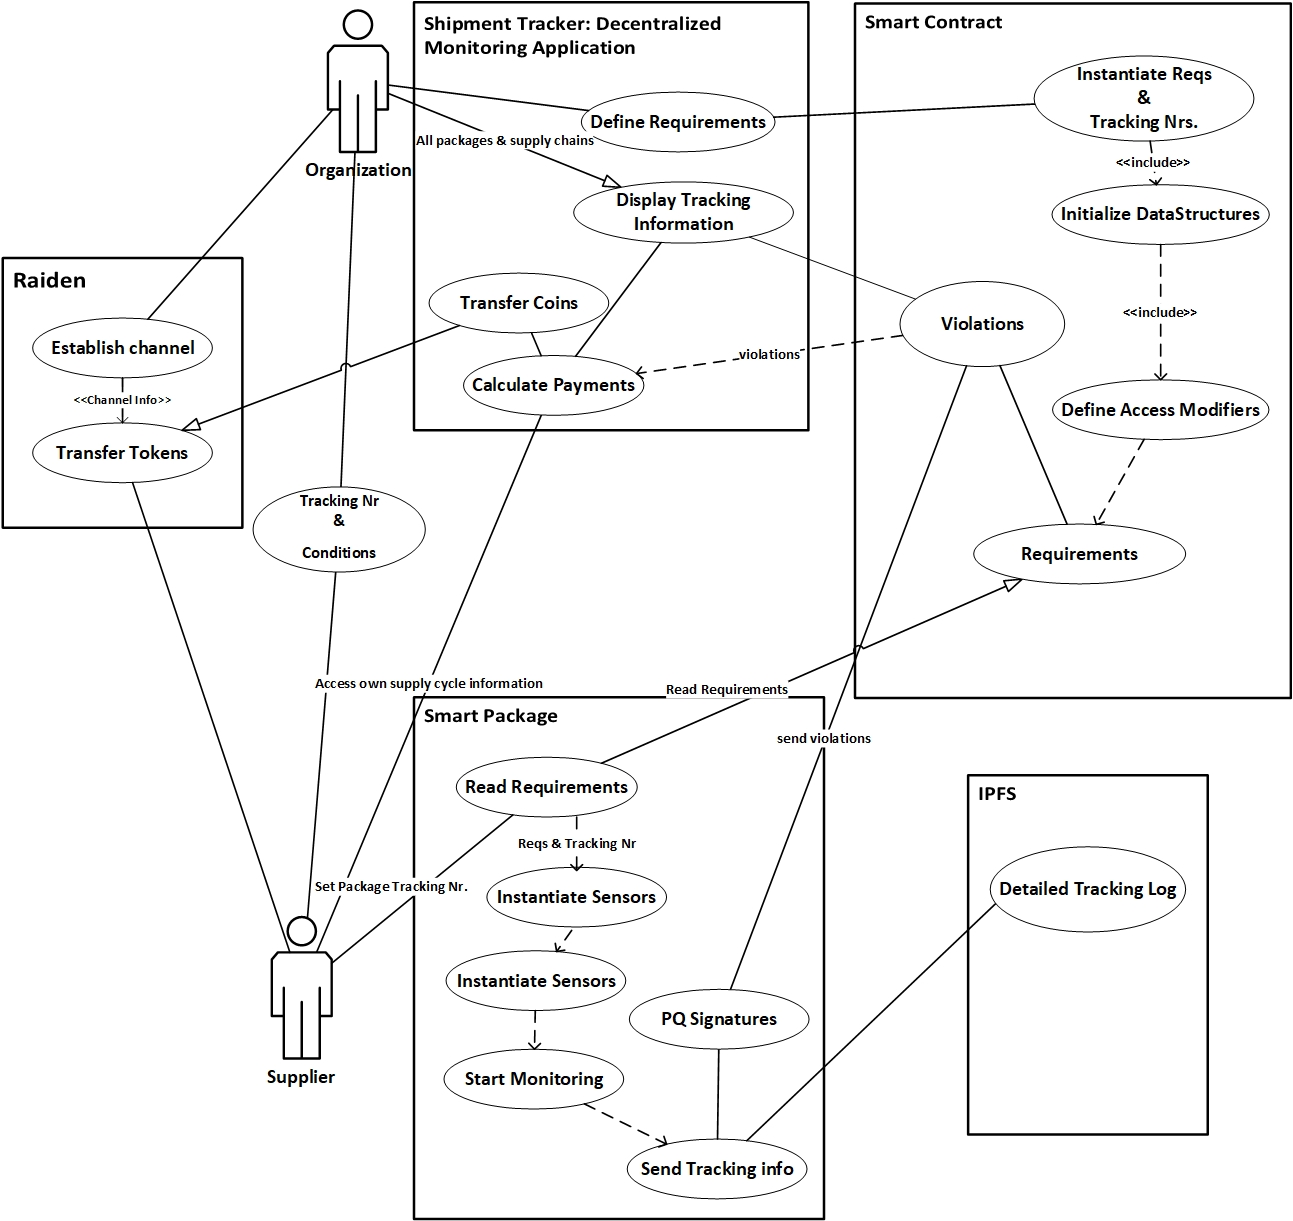
\includegraphics[width=170mm,scale=1]{figs/Abstractdesign}
	\caption{Shipment Tracker – Abstract Design}
	\label{fig:Abstractdesign}
\end{figure}
\clearpage




\subsection{Architecture - Block Diagram Overview}
Figure \ref{fig:ArchitectureBD} shows the architectural overview of our system. This system is composed of three high level components: Master Node (see \ref{MasterNode}), IoT Node (see \ref{IoTNode}) and Smart Contract (see \ref{ST-SC}). The Master Node provides an overview of the entire supply chain including activities within individual supply lines. It also handles compensation and payments to suppliers. The IoT Nodes monitor package conditions and communicates logging and tracking data with Smart Contract and IPFS. The Smart Contract provides function and logic to serve as a trustless bridge between Master Node and IoT Node. The Master Node queries the smart contract to get IPFS log locations and shipping violations.
\begin{figure}[h]
	\centering
    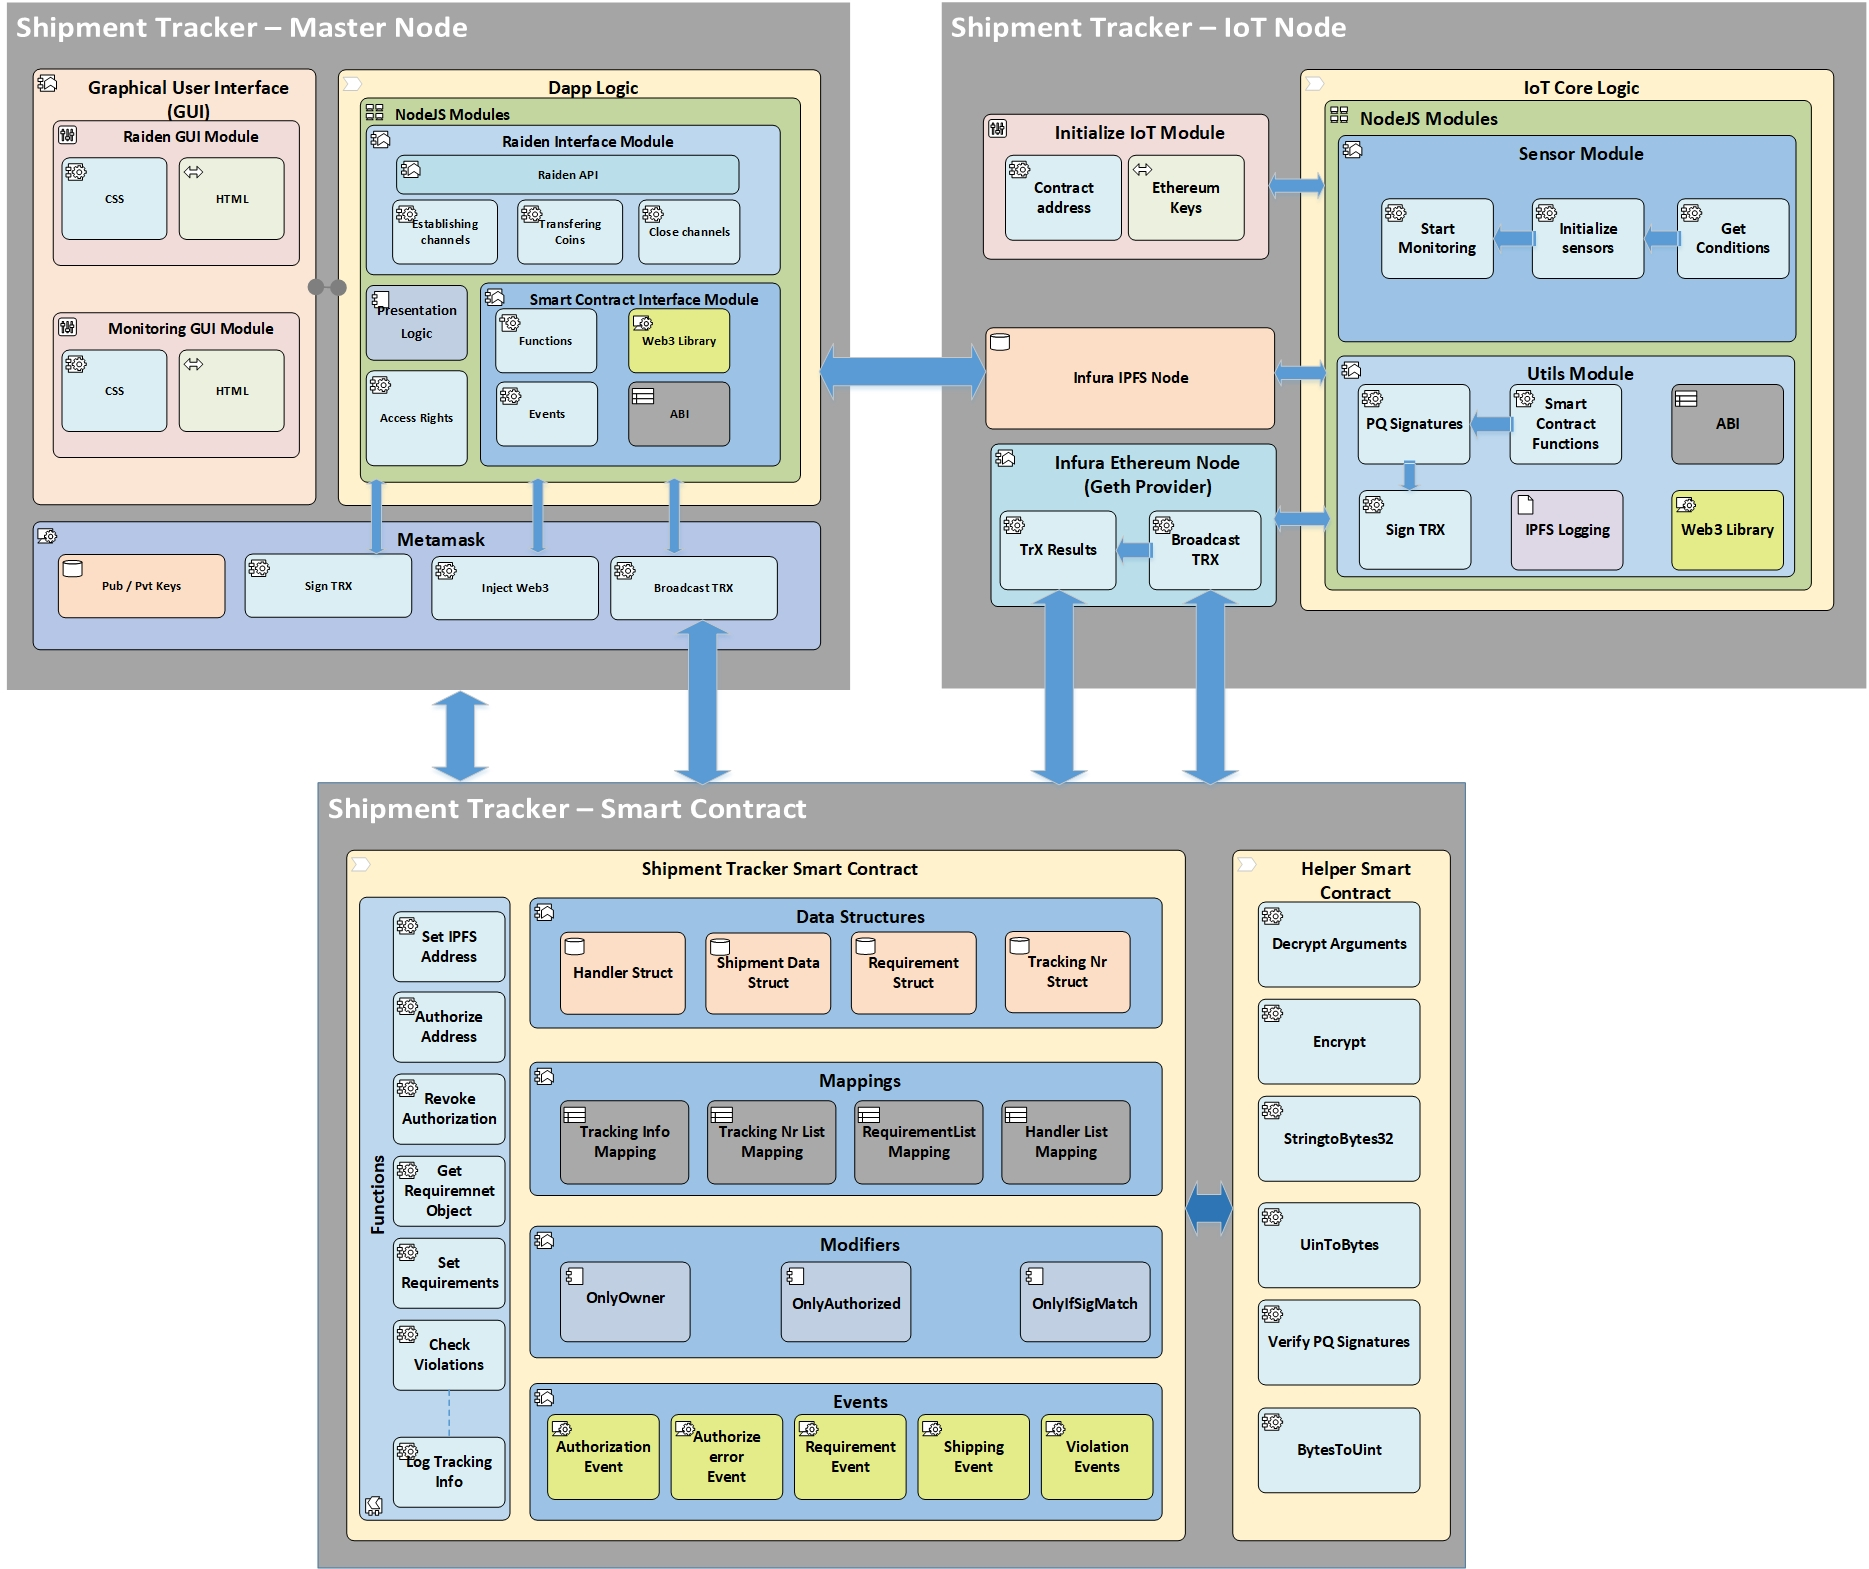
\includegraphics[width=180mm,scale=1]{figs/Blockdiagram}
	\caption{Shipment Tracker – System Block Diagram}
	\label{fig:ArchitectureBD} 
\end{figure}
\clearpage
\subsection{System Components} \label{SysComp} 
\subsubsection{Decentralized Monitoring Application - Master Node} \label{MasterNode} 
Figure \ref{fig:ArchitectureMN} details the architecture of the Master Node. This component contains the main decentralized application for monitoring all shipments across multiple supply lines. Its primary intent is to provide administrators or managers a comprehensive overview of the entire supply chain. Ethereum public key serves as the main access control mechanism in this module. It uses the public key to determine which processes or supply lines a user can view or access. The access rights are defined and stored in the Smart Contract. The Master Node has two main sub modules. One module deals with payments and payments channels. This module relies on Raiden (see \ref{raiden}) API to establish payment channels. Raiden client must be running and fully synced with Ethereum blockchain for this module to function. The second module interfaces with the Shipment Tracker Smart Contract deployed on the Ethereum blockchain. The associated GUI for this module (see fig \ref{fig:ArchitectureMN}) can be used to define requirements and constraints on shipments and packages, that must be followed by suppliers and shippers. This module uses web3 JavaScript library and MetaMask browser extension to broadcast transactions to the Ethereum Blockchain. MetaMask allows us to run our Dapp Master Node without running a full Ethereum Node. The implementation details and functions of each submodule in Master Node are described in \ref{IMN}. 

\begin{figure}[h]
	\centering
    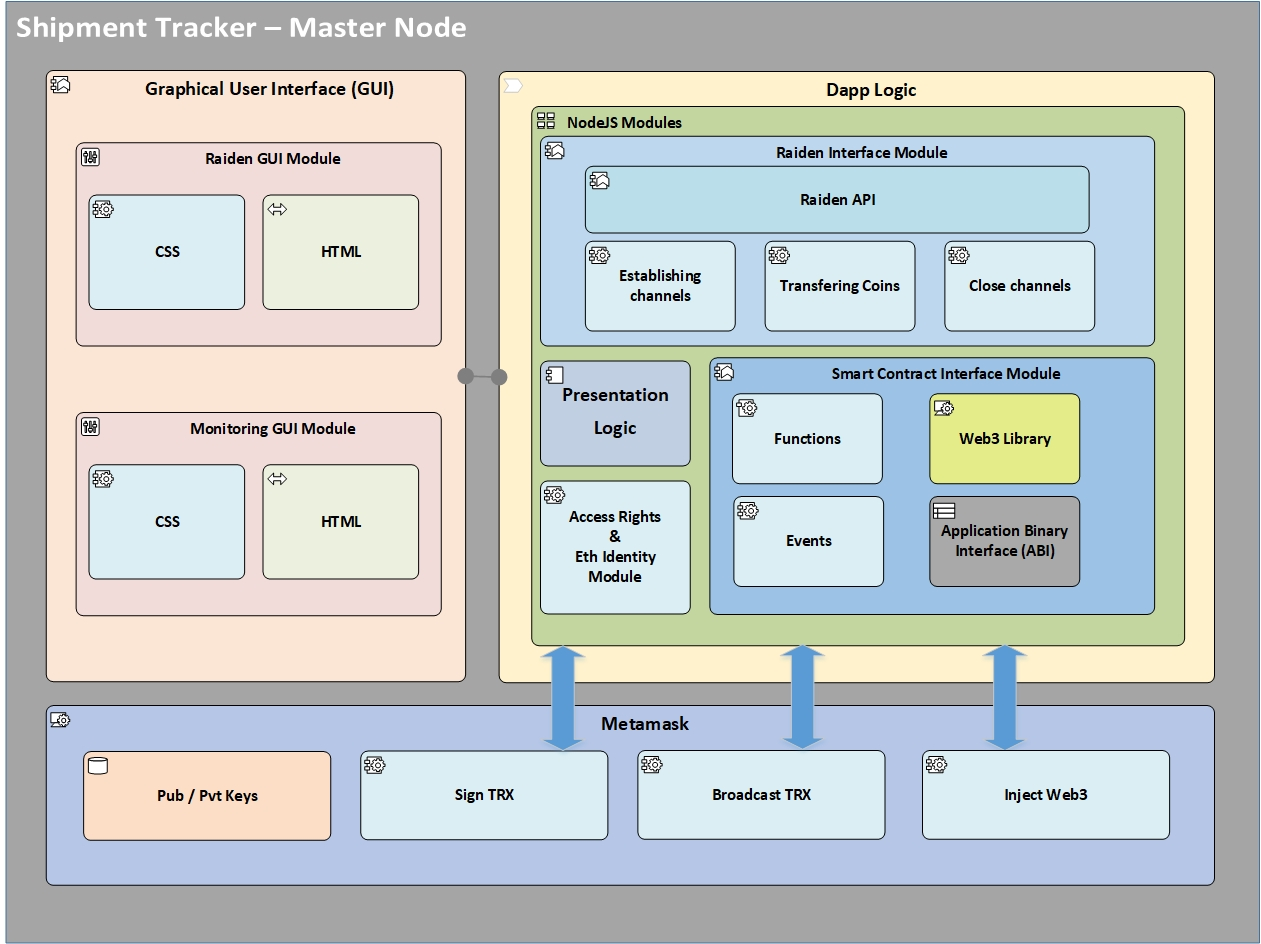
\includegraphics[width=160mm,scale=1]{figs/MasterNode-BD}
	\caption{Master Node – Block Diagram}
	\label{fig:ArchitectureMN} 
\end{figure}
\clearpage
\subsubsection{IoT Powered Smart Packages - IoT Nodes} \label{IoTNode} 
Figure \ref{fig:ArchitectureIoT} shows the architecture of IoT Nodes. An IoT Node is an embedded device with various sensors attached to monitor shipment/package conditions. IoT core logic is sub divided into three main modules: Initialization Module, Sensor Module and Utils Module. The Initialization Module is responsible for bootstrapping the device at the start of each new shipping cycle. It sets the shipment tracking number, contract address, monitoring and logging intervals and initializes the attached sensors. The device enters the monitoring phase after initialization is complete. In this phase the IoT Node first contacts the Shipment Tracker Smart Contract to get a list of conditions associated with the current tracking number. It then starts monitoring functions to periodically check that no condition gets violated. If any violations are found, it sends them to the Smart Contract to be permanently recorded on the blockchain. In order to communicate with the blockchain we must have access to an Ethereum client. IoT Nodes use the remote Ethereum Geth client provided by Infura. The client provided by Infura is not a wallet and it does not store keys or sign transaction. It expects that any state altering transactions that it receives are already signed. IoT Node uses the Utils Module to send signed transactions to the Geth client hosted on Infura. The Utils Module is also responsible for storing shipping logs on the IPFS Network.  The implementation details of the IoT Node are explained in \ref{IoT-Nodes}.

\begin{figure}[h]
	\centering
    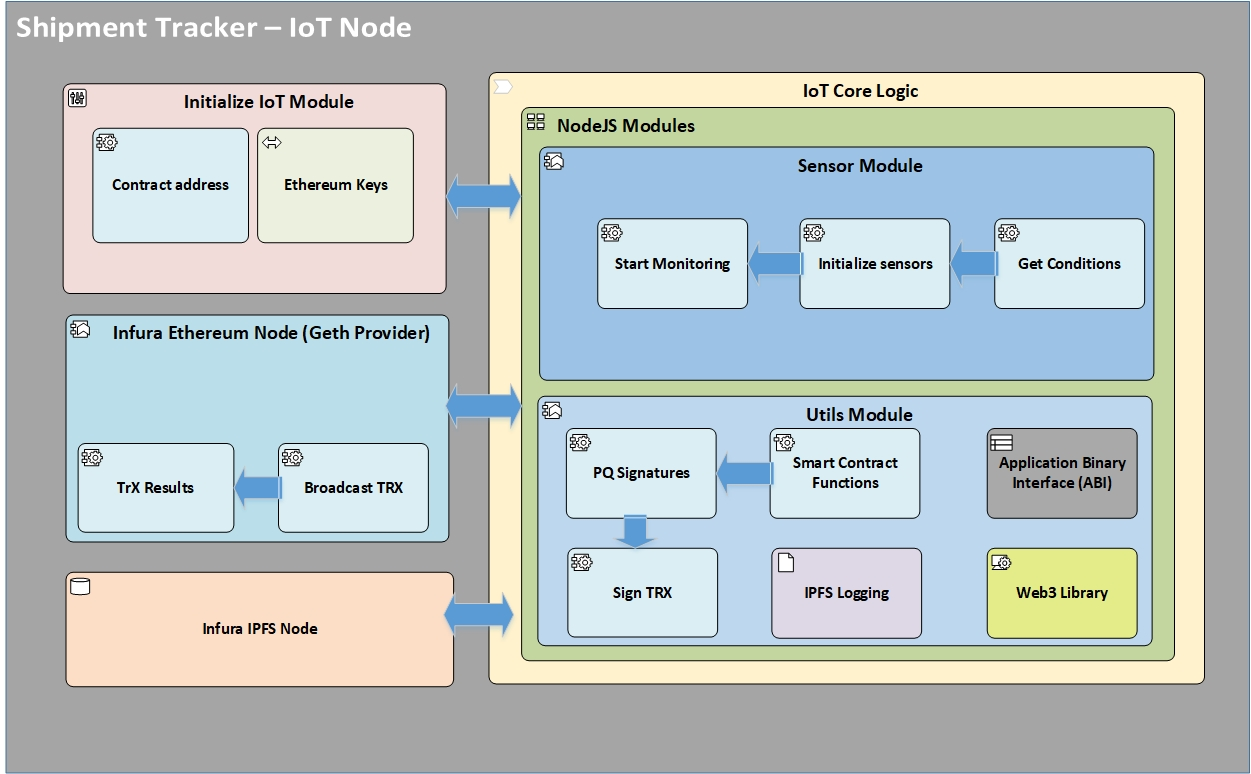
\includegraphics[width=180mm,scale=1]{figs/IoTNode-BD}
	\caption{IoT Node – Block Diagram}
	\label{fig:ArchitectureIoT} 
\end{figure}
\clearpage

\subsubsection{Shipment Tracker - Smart Contract} \label{ST-SC} 
The shipment Tracker contract is composed of several components as shown in figure \ref{fig:ArchitectureSC}. The functional logic of this contract is broken into several public, private and internal functions. Details of some of the important functional components is given in \ref{ST-SmartContract}.  The contract defines several data structures to store logical data. Shipment data and violations sent by the IoT Node are stored in ShipmentData (see \ref{ST-SmartContract}) structure. Requirements for individual shipping cycles are held in Requirements (see \ref{ST-SmartContract}) structure and the list of authorized handlers for individual shipments are saved in the Handler (see \ref{ST-SmartContract}) structure. Solidity Modifiers are used for modifying function behavior based on pre-defined condition. In our contract modifiers are used for restricting access to certain functions and mappings. Only authorized personal or devices are allowed to access these mappings. We use the modifier OnlyIfSigMatch to insure that data sent by IoT devices is correctly signed by the Post Quantum key of the current shipper. Only verified violations are added to the blockchain. Events are used to inform the Master Node, if any state altering function was executed by the Smart Contract. The final component in figure \ref{fig:ArchitectureSC} is the library contract helper.sol. In Solidity library contracts are singletons which do not store anything and can be called by any contract to extend their functionality. We developed library contract to handle Post Quantum Signature Verification. The main contract calls this library contract to verify PQ signatures. The library driven development helps to make our Smart Contract modular. It also insures that the main contract does not exceed the block limit. The current block limit on Ethereum main net is eight million gwei.  
\begin{figure}[h]
	\centering
    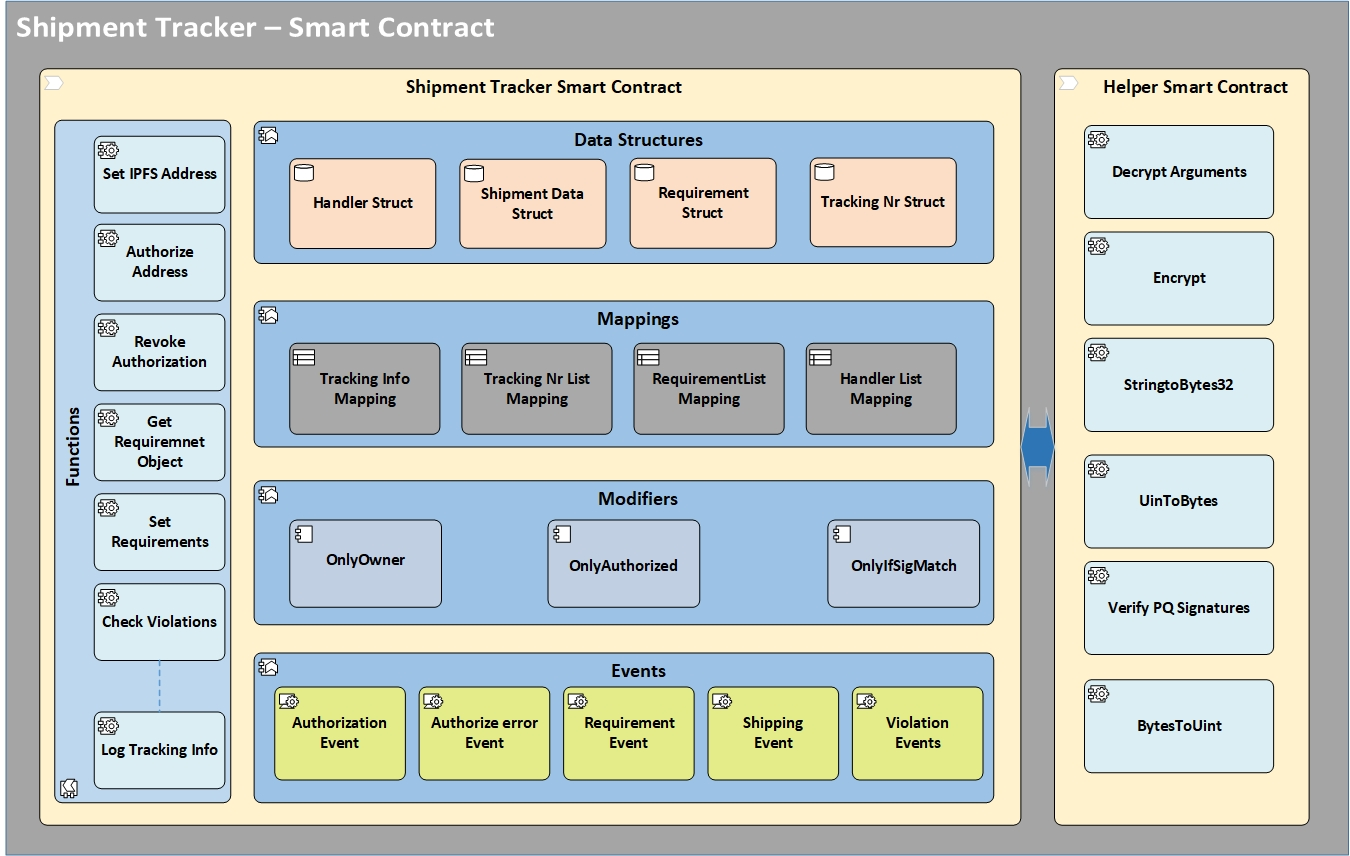
\includegraphics[width=170mm,scale=1]{figs/SC-BD}
	\caption{Smart Contract – Block Diagram}
	\label{fig:ArchitectureSC} 
\end{figure}
\clearpage



%\subsubsection{Post Quantum Module}

%say that a shipper key will be transferred when a new shipper scans the package

%\subsection{Initial Architecture}

%mention that initially each delivery cycle was going to be a single contract deployed, however this would generate lots of segregated contracts to keep track of. plus it will be very expensive in terms of operations, deployement and mantanence on public blockchain like ethereum where user pays for gas. refer to gas consumtion testing section. May even require full time blockchain developers to be able to make changes and improvements to exisiting contract templates.
%Advantage would be easiser to deal with custom situations and supply chain processes
%costs of operations would scale with ethereum prices. would make budget planning extremly difficult for organizations

%using such a systemn would create large number segregated databases which would %quickly become unmanagable for large organizations in the events of audits and analytics puposes. This will need created new buisness and IT systems for gathering managing organizing and managing distributed supply chain information.  We want distribution and redundancy of actual data and logic without adding operational overhead in terms of DB consolidtion and management on organizational level processes. The blockchain is providing an adequate solution for taking care of distribution and redundancy, Hence it was decided that it would be more worth while to invest efforts in developing a system which could serve as one generic smart contract for most of organizational needs. refer to section below.  